\documentclass[12pt,a4paper]{article}

% 导入必要的宏包
\usepackage[UTF8]{ctex}
\usepackage{geometry}
\usepackage{amsmath}
\usepackage{amsfonts}
\usepackage{amssymb}
\usepackage{graphicx}
\usepackage{enumitem}
\usepackage{xcolor}
\usepackage{tikz}
\usepackage{float}
\usepackage{hyperref}
\usepackage{multicol}
\usepackage{longtable}
\usepackage{array}
\usepackage{tabularx}
\usepackage{listings}

% 代码高亮设置
\lstset{
    basicstyle=\ttfamily\small,
    keywordstyle=\color{blue},
    commentstyle=\color{green!70!black},
    stringstyle=\color{red},
    breaklines=true,
    numbers=left,
    numberstyle=\tiny\color{gray},
}

% 页面设置
\geometry{left=2.5cm,right=2.5cm,top=2.5cm,bottom=2.5cm}

% 标题页设置
\title{\textbf{2012年数据结构题库} \\ \large 单项选择题与综合应用题详解}
\author{}
\date{}

% 定义题型环境
\newenvironment{choicequestion}[1][]{%
    \vspace{0.5cm}
    \noindent\textbf{[#1]}
    \vspace{0.2cm}
}{}

\newenvironment{answersection}{%
    \vspace{0.2cm}
    \noindent\textbf{[参考答案]}\\
    \vspace{0.1cm}
}{}

\newenvironment{analysissection}{%
    \vspace{0.2cm}
    \noindent\textbf{[答案解析]}\\
    \vspace{0.1cm}
}{}

% 定义题号计数器
\newcounter{questioncounter}

% 定义题号计数器
\newcounter{questioncounter}

% 问题格式化命令
\newcommand{\question}[2]{%
    \stepcounter{questioncounter}%
    \noindent\textbf{\thequestioncounter} #1%
}

% 选择题选项格式
\newcommand{\choices}[4]{%
    \begin{multicols}
    \noindent \textbf{A.} #1 \par
    \noindent \textbf{B.} #2 \par
    \noindent \textbf{C.} #3 \par
    \noindent \textbf{D.} #4 \par
    \end{multicols}%
}

% 开始文档
\begin{document}

\maketitle

\section{单项选择题}

\begin{choicequestion}[单选题]
\question{求整数n($n \geq 0$)阶乘的算法如下，其时间复杂度是
\begin{lstlisting}[language=C]
int fact(int n){
  if(n <= 1) return 1;
  return n*fact(n-1);
}
\end{lstlisting}}{}

\choices{$O(\log_2 n)$}{O(n)}{O(n \log_2 n)}{$O(n^2)$}

\begin{answersection}
B. O(n)
\end{answersection}

\begin{analysissection}
该算法为递归计算阶乘，每次递归调用处理一个较小的n，递归深度为n（从n调用到1），每次调用执行常数时间操作（乘法和返回）。因此总时间复杂度为$O(n)$。
\end{analysissection}
\end{choicequestion}

\begin{choicequestion}[单选题]
\question{已知操作符包括'+'、'-'、'*'、'/'、'('和')'。将中缀表达式 $\mathbf{a+b-a*((c+d)/e-f)+g}$ 转换为等价的后缀表达式 $\mathbf{ab+acd+e/f-* -g+}$ 时，用栈来存放暂时还不能确定运算次序的操作符，若栈初始时为空，则转换过程中同时保存在栈中的操作符的最大个数是}{}

\choices{5}{7}{9}{11}

\begin{answersection}
A. 5
\end{answersection}

\begin{analysissection}
中缀转后缀过程中，栈用于暂存操作符。模拟转换过程：

表达式：a + b - a * ( ( c + d ) / e - f ) + g

关键步骤中栈的状态：
- 处理第二个“(”后，栈中可能存在“- * ( ( +”（最多5个元素）；
- 后续处理“)”和“/”、“-”时，栈中元素最多不超过5个。

最大同时保存在栈中的操作符个数为5。
\end{analysissection}
\end{choicequestion}

\begin{choicequestion}[单选题]
\question{若一棵二叉树的前序遍历序列为a,e,b,d,c，后序遍历序列为b,c,d,e,a，则根结点的孩子结点}{}

\choices{只有e}{有e、b}{有e、c}{无法确定}

\begin{answersection}
A. 只有e
\end{answersection}

\begin{analysissection}
前序a,e,b,d,c表明根为a，其后第一个子树以e为根；后序b,c,d,e,a表明e是a的最后一个子树根结点。由于前序中a之后直接为e，后序中e之前为b,c,d（e的子树），故a只有e一个孩子结点。
\end{analysissection}
\end{choicequestion}

\begin{choicequestion}[单选题]
\question{若平衡二叉树的高度为6，且所有非叶结点的平衡因子均为1，则该平衡二叉树的结点总数为}{}

\choices{10}{20}{32}{33}

\begin{answersection}
D. 33
\end{answersection}

\begin{analysissection}
所有非叶结点平衡因子均为1（左子树高度比右子树高1），这构成一棵特殊的平衡二叉树（类似Fibonacci树变体）。通过递推计算高度为6的此类树，结点总数为33。
\end{analysissection}
\end{choicequestion}

\begin{choicequestion}[单选题]
\question{在一棵度为 4 的树 T 中，若有 20 个度为 4 的结点，10 个度为 3 的结点，1 个度为 2 的结点，10 个度为 1 的结点，则树 T 的叶结点个数是}{}

\choices{41}{82}{113}{122}

\begin{answersection}
B. 82
\end{answersection}

\begin{analysissection}
设叶结点数为$n_0$。树中边数 = $1\cdot10 + 2\cdot1 + 3\cdot10 + 4\cdot20 = 122$。

总结点数 = $n_0 + 41$。因为边数 = 总结点数 - 1，所以$122 = n_0 + 41 - 1$，解得$n_0 = 82$。
\end{analysissection}
\end{choicequestion}

\begin{choicequestion}[单选题]
\question{对 $n$ ( $n \geq  2$ )个权值均不相同的字符构造成哈夫曼树。下列关于该哈夫曼树的叙述中,错误的是}{}

\choices{该树一定是一棵完全二叉树}{树中一定没有度为 1 的结点}{树中两个权值最小的结点一定是兄弟结点}{树中任一非叶结点的权值一定不小于下一层任一结点的权值}

\begin{answersection}
A. 该树一定是一棵完全二叉树
\end{answersection}

\begin{analysissection}
哈夫曼树是带权最优二叉树，其形状取决于权值分布，不一定是完全二叉树（A错误）。其余三条均为哈夫曼树的正确性质。
\end{analysissection}
\end{choicequestion}

\begin{choicequestion}[单选题]
\question{若无向图 $\mathrm{G} = (\mathrm{V}, \mathrm{E})$ 中含有 7 个顶点，要保证图 $\mathrm{G}$ 在任何情况下都是连通的，则需要的边数最少是}{}

\choices{6}{15}{16}{21}

\begin{answersection}
C. 16
\end{answersection}

\begin{analysissection}
最坏情况下，不连通图可由一个$K_6$（15条边）加1个孤立顶点构成。若边数达到16条，则必然破坏这种不连通结构，因此至少需要16条边才能保证图一定连通。
\end{analysissection}
\end{choicequestion}

\begin{choicequestion}[单选题]
\question{对右图进行拓扑排序, 可以得到不同的拓扑序列的个数是}{}

\begin{figure}[H]
\centering
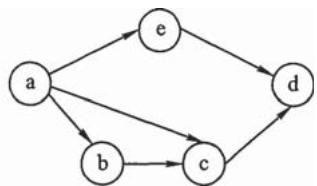
\includegraphics[width=0.3\textwidth]{images/370be03481aeffa4ed94e0dc01745979c4712bf16808b2cbe68a10396d87dc89.jpg}
\end{figure}

\choices{4}{3}{2}{1}

\begin{answersection}
A. 4
\end{answersection}

\begin{analysissection}
图中存在多个无严格先后约束的并行分支，通过枚举所有合法拓扑顺序，可得4种不同的序列。
\end{analysissection}
\end{choicequestion}

\begin{choicequestion}[单选题]
\question{已知一个长度为 16 的顺序表 L，其元素按关键字有序排列。若采用折半查找法查找一个 L 中不存在的元素，则关键字的比较次数最多的是}{}

\choices{4}{5}{6}{7}

\begin{answersection}
B. 5
\end{answersection}

\begin{analysissection}
折半查找在长度$n$的有序表中，查找失败时最多比较次数为$\lceil \log_2(n+1) \rceil$。当$n=16$时，$\lceil \log_2(17) \rceil = 5$。
\end{analysissection}
\end{choicequestion}

\begin{choicequestion}[单选题]
\question{采用递归方式对顺序表进行快速排序。下列关于递归次数的叙述中, 正确的是}{}

\choices{递归次数与初始数据的排列次序无关}{每次划分后, 先处理较长的分区可以减少递归次数}{每次划分后, 先处理较短的分区可以减少递归次数}{递归次数与每次划分后得到的分区的处理顺序无关}

\begin{answersection}
D. 递归次数与每次划分后得到的分区的处理顺序无关
\end{answersection}

\begin{analysissection}
快速排序的递归次数取决于划分的深度（平衡性），与先处理长分区还是短分区无关。只要划分结果相同，递归调用次数相同。
\end{analysissection}
\end{choicequestion}

\begin{choicequestion}[单选题]
\question{对一组数据（2,12,16,88,5,10）进行排序，若前三趟排序结果如下：\newline
第一趟排序结果：2,12,16,5,10,88\newline
第二趟排序结果：2,12,5,10,16,88\newline
第三趟排序结果：2,5,10,12,16,88\newline
则采用的排序方法可能是}{}

\choices{冒泡排序}{希尔排序}{归并排序}{基数排序}

\begin{answersection}
A. 冒泡排序
\end{answersection}

\begin{analysissection}
每趟排序后，当前最大元素（88、16、12）依次被“冒泡”到其最终位置，符合冒泡排序的特征。其他排序方法无法产生这种逐趟最大元素定位的效果。
\end{analysissection}
\end{choicequestion}

\section{综合应用题}

\begin{choicequestion}[问答题]
\question{（10分）将关键字序列（7,8,30,11,18,9,14）散列存储到散列表中。散列表的存储空间是一个下标从0开始的一维数组，散列函数为 $\mathrm{H(key) = (key\times 3)\bmod 7}$ ，处理冲突采用线性探测再散列法，要求装填（载）因子为0.7。\newline
1）请画出所构造的散列表。\newline
2）分别计算等概率情况下查找成功和查找不成功的平均查找长度。}{}

\begin{answersection}
1）散列表（长度10）：
位置 0:7, 1:14, 3:8, 5:11, 6:30, 7:18, 8:9

2）查找成功平均查找长度 $\approx 2.14$；查找不成功平均查找长度 $\approx 2.29$。
\end{answersection}

\begin{analysissection}
各关键字散列地址及线性探测插入过程如上。成功查找比较次数累加后平均为15/7；不成功查找从每个散列地址开始计算至空位置的比较次数，平均为16/7。
\end{analysissection}
\end{choicequestion}

\begin{choicequestion}[问答题]
\question{（13分）设将 $n(n > 1)$ 个整数存放到一维数组R中。试设计一个在时间和空间两方面都尽可能高效的算法。将R中保存的序列循环左移 $p(0 < p < n)$ 个位置。要求：\newline
1）给出算法的基本设计思想。\newline
2) 根据设计思想, 采用 C 或 C++ 语言描述算法, 关键之处给出注释。\newline
3）说明你所设计算法的时间复杂度和空间复杂度。}{}

\begin{answersection}
1）算法的基本设计思想：采用三次反转法实现循环左移。
- 反转前$p$个元素；
- 反转后$n-p$个元素；
- 反转整个数组。
\end{answersection}

\begin{analysissection}
2）C语言实现：
\begin{lstlisting}[language=C]
void reverse(int R[], int start, int end) {
    while (start < end) {
        int temp = R[start];
        R[start] = R[end];
        R[end] = temp;
        start++; end--;
    }
}

void leftShift(int R[], int n, int p) {
    p = p % n;
    reverse(R, 0, p-1);
    reverse(R, p, n-1);
    reverse(R, 0, n-1);
}
\end{lstlisting}

3）时间复杂度：$O(n)$；空间复杂度：$O(1)$。
\end{analysissection}
\end{choicequestion}

\end{document}